\documentclass[tikz,border=5pt]{standalone}
\usepackage[T1]{fontenc}
\usepackage{lmodern,amsmath,amssymb}
\usetikzlibrary{arrows.meta,calc,positioning,fit,backgrounds,shapes.geometric,matrix,decorations.pathreplacing,patterns}
\definecolor{ink}{gray}{0.08}
\definecolor{wash}{gray}{0.965}
\definecolor{soft}{gray}{0.45}
\tikzset{box/.style={draw=ink,line width=.65pt,fill=white,align=center,inner sep=4pt,outer sep=0pt,font=\small},flow/.style={draw=ink,line width=.65pt,-{Latex[length=1.8mm,width=1.3mm]},rounded corners=2pt},annotation/.style={font=\scriptsize,text=soft,align=center},groupbox/.style={draw=soft,dashed,line width=.45pt,fill=wash}}
\begin{document}
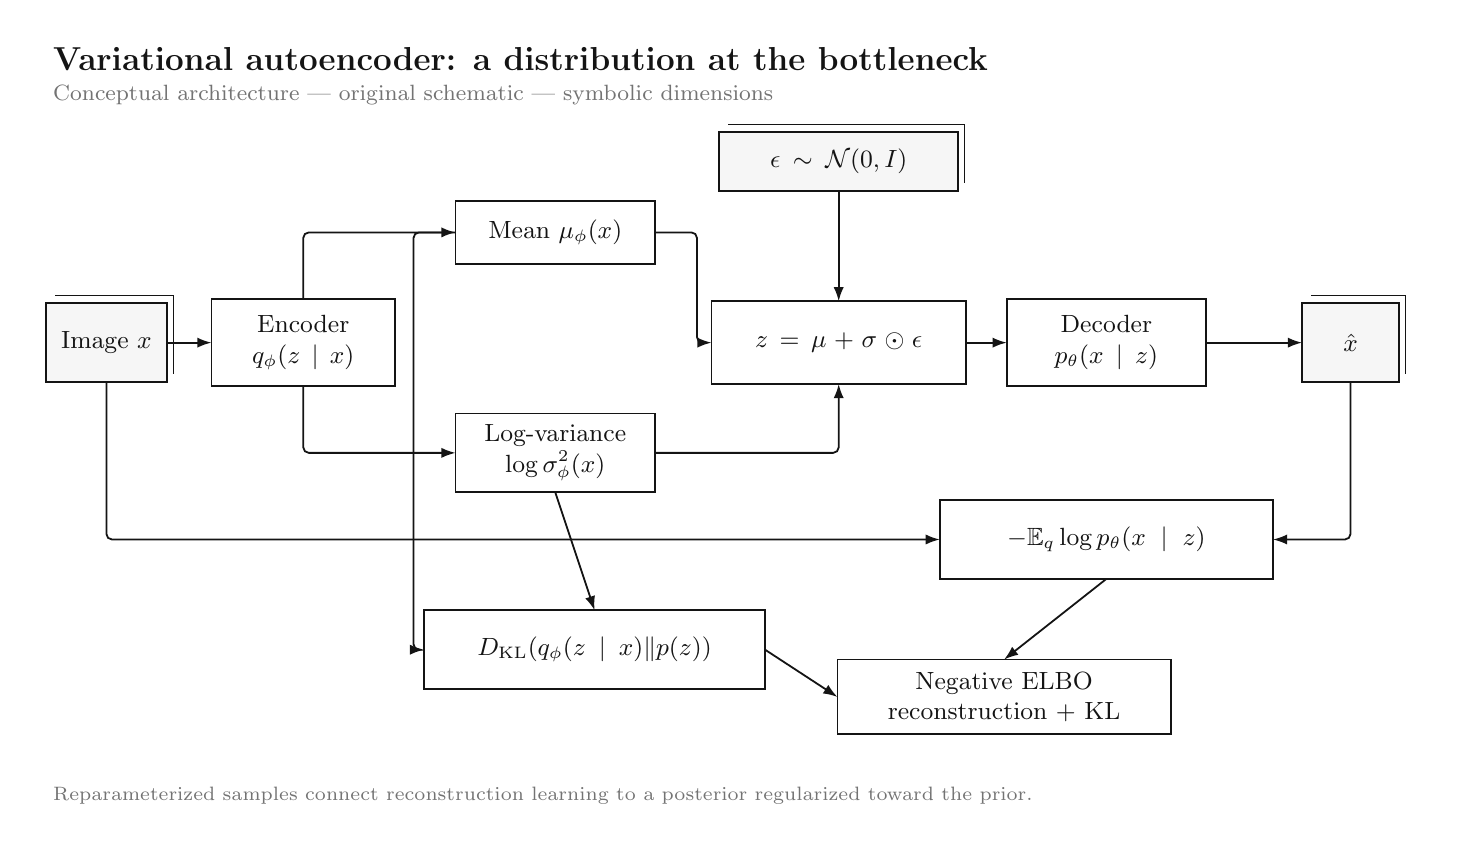
\begin{tikzpicture}[x=1cm,y=-1cm,font=\rmfamily,text=ink]

\path[use as bounding box] (0,0) rectangle (18,10);
\node[anchor=west,font=\large\bfseries] at (.2,.4) {Variational autoencoder: a distribution at the bottleneck};
\node[anchor=west,font=\footnotesize,text=soft] at (.2,.85) {Conceptual architecture | original schematic | symbolic dimensions};
\begin{pgfonlayer}{background}
\end{pgfonlayer}
\node[box,fill=wash,minimum width=1.5cm,minimum height=1.0cm,text width=1.25cm] (x) at (1.0,4.0) {Image $x$};
\draw[ink,line width=.4pt] (0.35,3.4) -- (1.85,3.4) -- (1.85,4.4);
\node[box,minimum width=2.3cm,minimum height=1.1cm,text width=2.05cm] (enc) at (3.5,4.0) {Encoder\\$q_\phi(z\mid x)$};
\node[box,minimum width=2.5cm,minimum height=0.8cm,text width=2.25cm] (mu) at (6.7,2.6) {Mean $\mu_\phi(x)$};
\node[box,minimum width=2.5cm,minimum height=1.0cm,text width=2.25cm] (lv) at (6.7,5.4) {Log-variance\\$\log\sigma_\phi^2(x)$};
\node[box,minimum width=3.2cm,minimum height=1.05cm,text width=2.95cm] (sample) at (10.3,4.0) {$z=\mu+\sigma\odot\epsilon$};
\node[box,fill=wash,minimum width=3.0cm,minimum height=0.75cm,text width=2.75cm] (noise) at (10.3,1.7) {$\epsilon\sim\mathcal N(0,I)$};
\draw[ink,line width=.4pt] (8.9,1.2249999999999999) -- (11.9,1.2249999999999999) -- (11.9,1.975);
\node[box,minimum width=2.5cm,minimum height=1.1cm,text width=2.25cm] (dec) at (13.7,4.0) {Decoder\\$p_\theta(x\mid z)$};
\node[box,fill=wash,minimum width=1.2cm,minimum height=1.0cm,text width=0.95cm] (out) at (16.8,4.0) {$\hat x$};
\draw[ink,line width=.4pt] (16.3,3.4) -- (17.500000000000004,3.4) -- (17.500000000000004,4.4);
\node[box,minimum width=4.3cm,minimum height=1.0cm,text width=4.05cm] (kl) at (7.2,7.9) {$D_{\rm KL}(q_\phi(z\mid x)\Vert p(z))$};
\node[box,minimum width=4.2cm,minimum height=1.0cm,text width=3.95cm] (rec) at (13.7,6.5) {$-\mathbb E_q\log p_\theta(x\mid z)$};
\node[box,minimum width=4.2cm,minimum height=0.95cm,text width=3.95cm] (obj) at (12.4,8.5) {Negative ELBO\\reconstruction + KL};
\begin{pgfonlayer}{background}
\draw[flow] (x.east) -- (enc.west);
\draw[flow] (enc.north) -- (3.5,2.6) -- (mu.west);
\draw[flow] (enc.south) -- (3.5,5.4) -- (lv.west);
\draw[flow] (mu.east) -- (8.5,2.6) -- (8.5,4.0) -- (sample.west);
\draw[flow] (lv.east) -- (10.3,5.4) -- (sample.south);
\draw[flow] (noise.south) -- (sample.north);
\draw[flow] (sample.east) -- (dec.west);
\draw[flow] (dec.east) -- (out.west);
\draw[flow] (lv.south) -- (kl.north);
\draw[flow] (mu.west) -- (4.9,2.6) -- (4.9,7.9) -- (kl.west);
\draw[flow] (out.south) -- (16.8,6.5) -- (rec.east);
\draw[flow] (x.south) -- (1.0,6.5) -- (rec.west);
\draw[flow] (kl.east) -- (obj.west);
\draw[flow] (rec.south) -- (obj.north);
\end{pgfonlayer}
\node[anchor=west,align=left,font=\scriptsize,text=soft,text width=17.6cm] at (.2,9.75) {Reparameterized samples connect reconstruction learning to a posterior regularized toward the prior.};
\end{tikzpicture}
\end{document}
